%
\documentclass [11pt,a4paper]{report}
\usepackage{csquotes}
\usepackage{biblatex}
\addbibresource{bibliography.bib}
\usepackage{url}
\usepackage{graphicx}
\usepackage{subfigure}

%
%
%   Define variables that are specific to this report:
%   --------------------------------------------------
%
\def\reporttitle{Theory of Rydberg Packets Immersed in Ultracold Gases}  % Title (name) of the report
\def\reportshorttitle{Rydberg Atom} % Short title (name)
%                                                   % of the report
\def\reportnumber{Rydberg Atom-zhonglin}     % Report identifier/number
\def\reportauthor{Lin Zhonglin} % Report author(s)
%
%
\def\solution{Solution to any}
\def\xyz{$x=y=z$}
%
%
%
%   Load the style file for technical reports of AMO group:
%   -------------------------------------------------------
%
\input{/Users/JohnnyLin/Desktop/HumboldtProgram/HU_AMO_report_template/amo_technical_reports.sty}    % Load style template file
%
%======================================================================
%
%
\begin{document}

\firstpage%
%

\msk\noindent%

%
%
%   Input of the content of the technical report starts here:
%   =========================================================
%
%
\section{Summary}
\label{sec:summary}
The overall idea of the project is to use Yulian's code on hydrogen molecule system to investigate how a Rydberg state around one hydrogen nucleus behaves as another Rydberg state around a secibd hydrogen nucleus separated signigicantly far apart evolves. The intuitive expectation is that the two Rydberg states should evolve synchronously following classical-like orbits.

The project is to be approached through the following steps:
\begin{enumerate}
  \item Investigate the convergence behavior of the hydrogen molecule code as basis and system parameters are varied.
  \item Settle on a resonable basis and investigate how an approaching (decreasing internuclei distance) second nucleus affects a Rydberg state (i.e. hydrogen ion system).
  \item With the same basis, investigate how a Rydberg state around one hydrogen nucleus behaves as another Rydberg state around another hydrogen nucleus separated signigicantly far apart.
\end{enumerate}

My project ran out of time at the second step. This report contains relevant theory background, code documentation and most of the results I obtained such that anyone wishing to continue with the project will find them helpful.

%
%---------------------------------------------------------------------
%
\section{Updates (in inverse chronological order)}
\label{sec:updates}

\begin{description}
   \item[4.8.2023:] Start writing first draft by transferring over results and discussions from notion
\end{description}


%
%---------------------------------------------------------------------
%
\section{Theory Background on Numerical Solution of Schrödinger equation}
\label{sec:theory}
The Schrödinger equation which is the main equation in atomic, molecular and optical (AMO) physics can be solved analytically only in a few cases. In order to solve most of the occurring problems one must resort to approximation methods such as perturbation theory and variational methods. Among other implementations of variational principle, the usage of ``unphysical'' basis sets has become one of the most popular implementations. The Rayleigh-Ritz-Galerkin method allows to transform the solution of a differential equation into an algebraic eigenvalue problem, which then can be very efficiently solved using modern linear algebra packages. Numerous types of basis sets have been tested in the past but they can be classified into two groups, local and global basis sets. While the global basis functions, such as Slater type orbitals (STO) or Gaussians, are spread over the entire space domain, the local basis functions are non-zero only in a small part of the space domain. If these functions are piecewise polynomial, they are called finite elements or splines. Splines of various types have been used in numerical analysis for a long time, e.g. cardinal splines, Bézier splines, Hermite splines. All of them are $L^2$ integrable functions defined in a restricted space usually referred to as a box. In the box, a knot sequence is defined and the freedom to define the knots to suit the particular problem is one of the important advantages of the method. Every kind of splines is characterized by its degree, smoothness, and knot sequence and can be represented as a linear combination of basis splines (i.e. for a given degree, smoothness, and knot sequence its basis functions are non-zero on the shortest intervals compared to other spline basis sets) and B splines are positive defined functions. These two important properties are of great advantage in matrix calculations, since resulting matrices are sparse (often banded) and easier to diagonalize. \cite{YulianThesis}

Yulian's hydrogen atomic, one-electron molecular and two-electron molecular codes take in a basis and solves the respective Schrödinger equation numerically using the above approach. The code then outputs calculated eigenvalues and coefficients of the basis functions.

%
%---------------------------------------------------------------------
%
\section{Plan}
\label{sec:plan}
The overeall plan is as follow.
\begin{enumerate}
  \item First look for a set of basis and system parameters that both give satisfactory convergence and can be completed in reasonable run time. To do so, the second proton in the hydrogen molecule code is switched off to create a hydrogem atom system in Elliptical coordinate. Since the hydrogen atom system is analytically solvable, the numerical calculation results are compared with analytical value for convergence check. Meanwhile, single calculation runtime is restricted to below ten minutes for my project due to overall time constraint.
  \item Secdonly, switch on the second proton and decompose the single eletron state around one nucleus from previous step in the two nuclei system. Vary internuclei distance to see how the single electron state is affected by the presence of second proton.
  \item Thirdly, decompose two single electorn hydrogen ion state (around difference nuclei) in hydrogen molecule eigen states and see how they affect each other as they evolve in time.
\end{enumerate}

Note that we are generally interested in large internuclei separation such that the system resembles an optical lattice rather than a hydrogen molecule system which is analytically solvable. We are generally interested in Rydberg states which have large orbits and are expected to evolve in a classical-like orbit. Figure \ref{fig:plan} in Appendix contains a hand written note by Harkon that illustrates the steps.

%
%---------------------------------------------------------------------
%
\section{Basics of Yulian's code}
\label{sec:code_basics}
Some useful information:
\begin{enumerate}
  \item A succint documentation for using the codes is contained in directory: \url{///users/amo/group/programs/internal/AMO_TOOLS/AMO_TOOLS_HELP/manual.html}.
  \item Yulian's one-electron and two-electron codes are contained in directory: \url{AMO_TOOLS_WSER/ELECTR_STR/B_DAM_ECS}
  \item FORTRAN code is contained in directory: \url{/users/amo/group/programs/internal/AMO_TOOLS/AMO_TOOLS_CODE/ELECTR_STR/HSPH/code/}
\end{enumerate}

The FORTRAN procedure is run by a .csh c shell which calls multiple FORTRAN files. Note that the FORTRAN files need to compiled before being run. Refer to documentation given in point 1 for detailed instructions. The FORTRAN procedure takes in a particular input file template (unique to each FORTRAN procedure) and outputs in FORTRAN unformatted binary. For ease of running calculations and reading outputs, a python script alternative was developed by Nicole and me and was uploaded to \url{https://github.com/colaboy519/Humboldt_AMO_codes.git}. Tasks such as reading out the unformatted binary and plotting the output wave functions in Cartesian coordinate are also implemented in the python scripts. (although needing improvements here and there)

Read the README file for information on how to use the python scripts. Note that the python scripts can only be used in restricted scenarios and suggestions for further development are included as comments in the python scripts.

%
%---------------------------------------------------------------------
%
\section{Convergence Behavior Dependence on $N_x$}
\label{sec:N_x_convergence}
As a start, the basis and system parameters are varied to explore the behaviors of the code such as convergence behavior and run time behavior.

Basis and system parameters used are as follow:
\begin{figure}[H]
  \centering
  \includegraphics[width=.3\textwidth]{/Users/JohnnyLin/Desktop/HumboldtProgram/HU_AMO_techincal_report/basis.png}
  \caption{basis parameters}
  \label{basis_parameters}
\end{figure}

Some results are plotted below:

\subsection{Decreasing box size}
\label{sec:decreasing_box_size}
It can be seen from the plots below that as box size decreases, numerical eigevalues converges faster towards analytical values. The understanding is that with the box size sufficiently large compared to system dimension, smaller box size gives a denser basis function which bring about a faster convergence.

Another observation is that higher energy levels has faster convergence. The understanding is that higher energy states are spaerser and further away from nuclei hence require less dense basis functions for convergence.

\graphicspath{{/Users/JohnnyLin/Desktop/HumboldtProgram/HU_AMO_techincal_report/AMO_report_decreasing_box_size/}}
\begin{figure}[H]
  \centering
  \includegraphics[width=.7\textwidth]{x_max=400,R=1.png}
  \caption{$x_{max}=400,R=1$}
  \label{x_max=400,R=1}
\end{figure}

\begin{figure}[H]
  \centering
  \includegraphics[width=.7\textwidth]{x_max=300,R=1.png}
  \caption{$x_{max}=300,R=1$}
  \label{x_max=300,R=1}
\end{figure}

\begin{figure}[H]
  \centering
  \includegraphics[width=.7\textwidth]{x_max=200,R=1.png}
  \caption{$x_{max}=200,R=1$}
  \label{x_max=200,R=1}
\end{figure}

\begin{figure}[H]
  \centering
  \includegraphics[width=.7\textwidth]{x_max=100,R=1.png}
  \caption{$x_{max}=100,R=1$}
  \label{x_max=100,R=1}
\end{figure}

\begin{figure}[H]
  \centering
  \includegraphics[width=.7\textwidth]{x_max=50,R=1.png}
  \caption{$x_{max}=50,R=1$}
  \label{x_max=50,R=1}
\end{figure}

\begin{figure}[H]
  \centering
  \includegraphics[width=.7\textwidth]{x_max=25,R=1.png}
  \caption{$x_{max}=25,R=1$}
  \label{x_max=25,R=1}
\end{figure}

\begin{figure}[H]
  \centering
  \includegraphics[width=.7\textwidth]{x_max=10,R=1.png}
  \caption{$x_{max}=10,R=1$}
  \label{x_max=10,R=1}
\end{figure}


\subsection{Increasing internuclei distance}
It can be observed in the following plots that larger internuclei separation require more basis functions for convergence. The understanding is that since we are looking for spherically symmetric hydrogen atom states in an elliptical coordinate system, larger internuclei separation increases ellipticity of the coordinate system and hence makes convergence more difficult.

\graphicspath{{/Users/JohnnyLin/Desktop/HumboldtProgram/HU_AMO_techincal_report/AMO_report_increasing_R/}}
\begin{figure}[H]
  \centering
  \includegraphics[width=.7\textwidth]{x_max=100,R=2.png}
  \caption{$x_{max}=100,R=2$}
  \label{x_max=100,R=2}
\end{figure}

\begin{figure}[H]
  \centering
  \includegraphics[width=.7\textwidth]{x_max=100,R=3.png}
  \caption{$x_{max}=100,R=3$}
  \label{x_max=100,R=3}
\end{figure}

\begin{figure}[H]
  \centering
  \includegraphics[width=.7\textwidth]{x_max=100,R=10.png}
  \caption{$x_{max}=100,R=10$}
  \label{x_max=100,R=10}
\end{figure}


\subsection{Increasing internuclei distance and number of BSplines correspondingly}
Figure \ref{x_max=300,R=10} compared to Figure \ref{x_max=100,R=10} has tripled the box size. While Figure \ref{x_max=100,R=10} reaches convergence at about $N_X = 60$, Figure \ref{x_max=300,R=10} reaches convergence only at about $N_x = 150$. The understanding is as discussed in section \ref{sec:decreasing_box_size} that a larger box with the same number of basis functions results in a sparser grid that is worse for reaching convergence in calculation.


\graphicspath{{/Users/JohnnyLin/Desktop/HumboldtProgram/HU_AMO_techincal_report/AMO_report_increasing_R_Nx/}}
\begin{figure}[H]
  \centering
  \includegraphics[width=.7\textwidth]{x_max=300,R=10.png}
  \caption{$x_{max}=300,R=10$}
  \label{x_max=300,R=10}
\end{figure}

\begin{figure}[H]
  \centering
  \includegraphics[width=.7\textwidth]{x_max=300,R=20.png}
  \caption{$x_{max}=300,R=20$}
  \label{x_max=300,R=20}
\end{figure}

\begin{figure}[H]
  \centering
  \includegraphics[width=.7\textwidth]{x_max=300,R=30.png}
  \caption{$x_{max}=300,R=30$}
  \label{x_max=300,R=30}
\end{figure}

%
%---------------------------------------------------------------------
%
\section{Convergence Behavior Dependence on $R_{int}$}
\label{sec:R_int_convergence}
From Figure \ref{R_int1} alone, I was first mislead to think that the code fails to converge beyound a certain internuclei distance. However, Figure \ref{R_int1} shows that as internuclei distance increases there turns out to be a systematic upward shift of the eigen values. Hence, the code might continue to work with a relabeling of the eigen value levels. The exact details of this relabeling is left unhandelled.

\begin{figure}[H]
  \centering
  \includegraphics[width=.8\textwidth]{/Users/JohnnyLin/Desktop/HumboldtProgram/HU_AMO_techincal_report/AMO_report_figures/R_int1.png}
  \caption{numerical and analytical}
  \label{R_int1}
\end{figure}

\begin{figure}[H]
  \centering
  \includegraphics[width=\textwidth]{/Users/JohnnyLin/Desktop/HumboldtProgram/HU_AMO_techincal_report/AMO_report_figures/R_int2.png}
  \caption{numerical and analytical difference ratio}
  \label{R_int2}
\end{figure}



%
%---------------------------------------------------------------------
%
\section{Plotting Wave Functions}
\label{sec:plotting_wave_functions}
Although comparing the numerical eigenvalues with analytical eigenvalues can serve to some extent as an indication of convergence towards true values, a second verification would be to plot out the wavefunctions and see whether they are the expected analytical spherical harmonics.

The first step in plotting out the wave functions in Cartesian coordinate is to reproduce Figure 2.2 in \cite{YulianThesis}. Note that when plotting symmetric wave functions, some special treatment is needed as the code makes use of this symmetry to save computation.

In trying to reproduce Figure 2.2 in \cite{YulianThesis}, I was able to output the following plots using ECS12.py. There are still a few differences that I couldn't resolve. First there is vertical axis fipping with some figures which indicate a harmless phase factor. Secondly some plots are of by a small value in the x axis which I have not figured out why. My guess is that either the basis I used was not good enough or that the system I was plotting is different from the system Yulian used. However, as Yulian didnot provide information on the system corresponding to Figure 2.2 in \cite{YulianThesis}, I couldnot check. Thirdly, for instance, figure \ref{fig:3g} seems to deviate from Yulian's plot by just a flipping of half the curve in the middle. However, I have not figured why and also still cannot resolve the x axis shifting issue. This is left to anyone following up with the project in the future.

\begin{figure}[H]
  \centering
  \subfigure[1u-xi]{\includegraphics[width=0.4\linewidth]{/Users/JohnnyLin/Desktop/HumboldtProgram/HU_AMO_techincal_report/AMO_report_figures_wavefunctions/1u-xi.png}}
  \hfill
  \subfigure[1u-eta]{\includegraphics[width=0.4\linewidth]{/Users/JohnnyLin/Desktop/HumboldtProgram/HU_AMO_techincal_report/AMO_report_figures_wavefunctions/1u-eta.png}}
  \caption{1u}
  \label{fig:1u}
\end{figure}

\begin{figure}[H]
    \centering
    \subfigure[1g-xi]{\includegraphics[width=0.4\linewidth]{/Users/JohnnyLin/Desktop/HumboldtProgram/HU_AMO_techincal_report/AMO_report_figures_wavefunctions/1g-xi.png}}
    \hfill
    \subfigure[1g-eta]{\includegraphics[width=0.4\linewidth]{/Users/JohnnyLin/Desktop/HumboldtProgram/HU_AMO_techincal_report/AMO_report_figures_wavefunctions/1g-eta.png}}
    \caption{1g}
    \label{fig:1g}
\end{figure}

\begin{figure}[H]
    \centering
    \subfigure[2u-xi]{\includegraphics[width=0.4\linewidth]{/Users/JohnnyLin/Desktop/HumboldtProgram/HU_AMO_techincal_report/AMO_report_figures_wavefunctions/2u-xi.png}}
    \hfill
    \subfigure[2u-eta]{\includegraphics[width=0.4\linewidth]{/Users/JohnnyLin/Desktop/HumboldtProgram/HU_AMO_techincal_report/AMO_report_figures_wavefunctions/2u-eta.png}}
    \caption{2u}
    \label{fig:2u}
\end{figure}

\begin{figure}[H]
    \centering
    \subfigure[2g-xi]{\includegraphics[width=0.4\linewidth]{/Users/JohnnyLin/Desktop/HumboldtProgram/HU_AMO_techincal_report/AMO_report_figures_wavefunctions/2g-xi.png}}
    \hfill
    \subfigure[2g-eta]{\includegraphics[width=0.4\linewidth]{/Users/JohnnyLin/Desktop/HumboldtProgram/HU_AMO_techincal_report/AMO_report_figures_wavefunctions/2g-eta.png}}
    \caption{2g}
    \label{fig:2g}
\end{figure}

\begin{figure}[H]
    \centering
    \subfigure[3u-xi]{\includegraphics[width=0.4\linewidth]{/Users/JohnnyLin/Desktop/HumboldtProgram/HU_AMO_techincal_report/AMO_report_figures_wavefunctions/3u-xi.png}}
    \hfill
    \subfigure[3u-eta]{\includegraphics[width=0.4\linewidth]{/Users/JohnnyLin/Desktop/HumboldtProgram/HU_AMO_techincal_report/AMO_report_figures_wavefunctions/3u-eta.png}}
    \caption{3u}
    \label{fig:3u}
\end{figure}

\begin{figure}[H]
    \centering
    \subfigure[3g-xi]{\includegraphics[width=0.4\linewidth]{/Users/JohnnyLin/Desktop/HumboldtProgram/HU_AMO_techincal_report/AMO_report_figures_wavefunctions/3g-xi.png}}
    \hfill
    \subfigure[3g-eta]{\includegraphics[width=0.4\linewidth]{/Users/JohnnyLin/Desktop/HumboldtProgram/HU_AMO_techincal_report/AMO_report_figures_wavefunctions/3g-eta.png}}
    \caption{3g}
    \label{fig:3g}
\end{figure}


%
%---------------------------------------------------------------------
%
\section{Remaining Work}
\label{sec:remaining_work}
Referring back to section \ref{sec:plan}, I was only able to reach the first step. Someone interested should be able to pick up the project from second step onward pretty quickly.


%
%=====================================================================
%
\appendix

\begin{figure}[H]
  \centering
  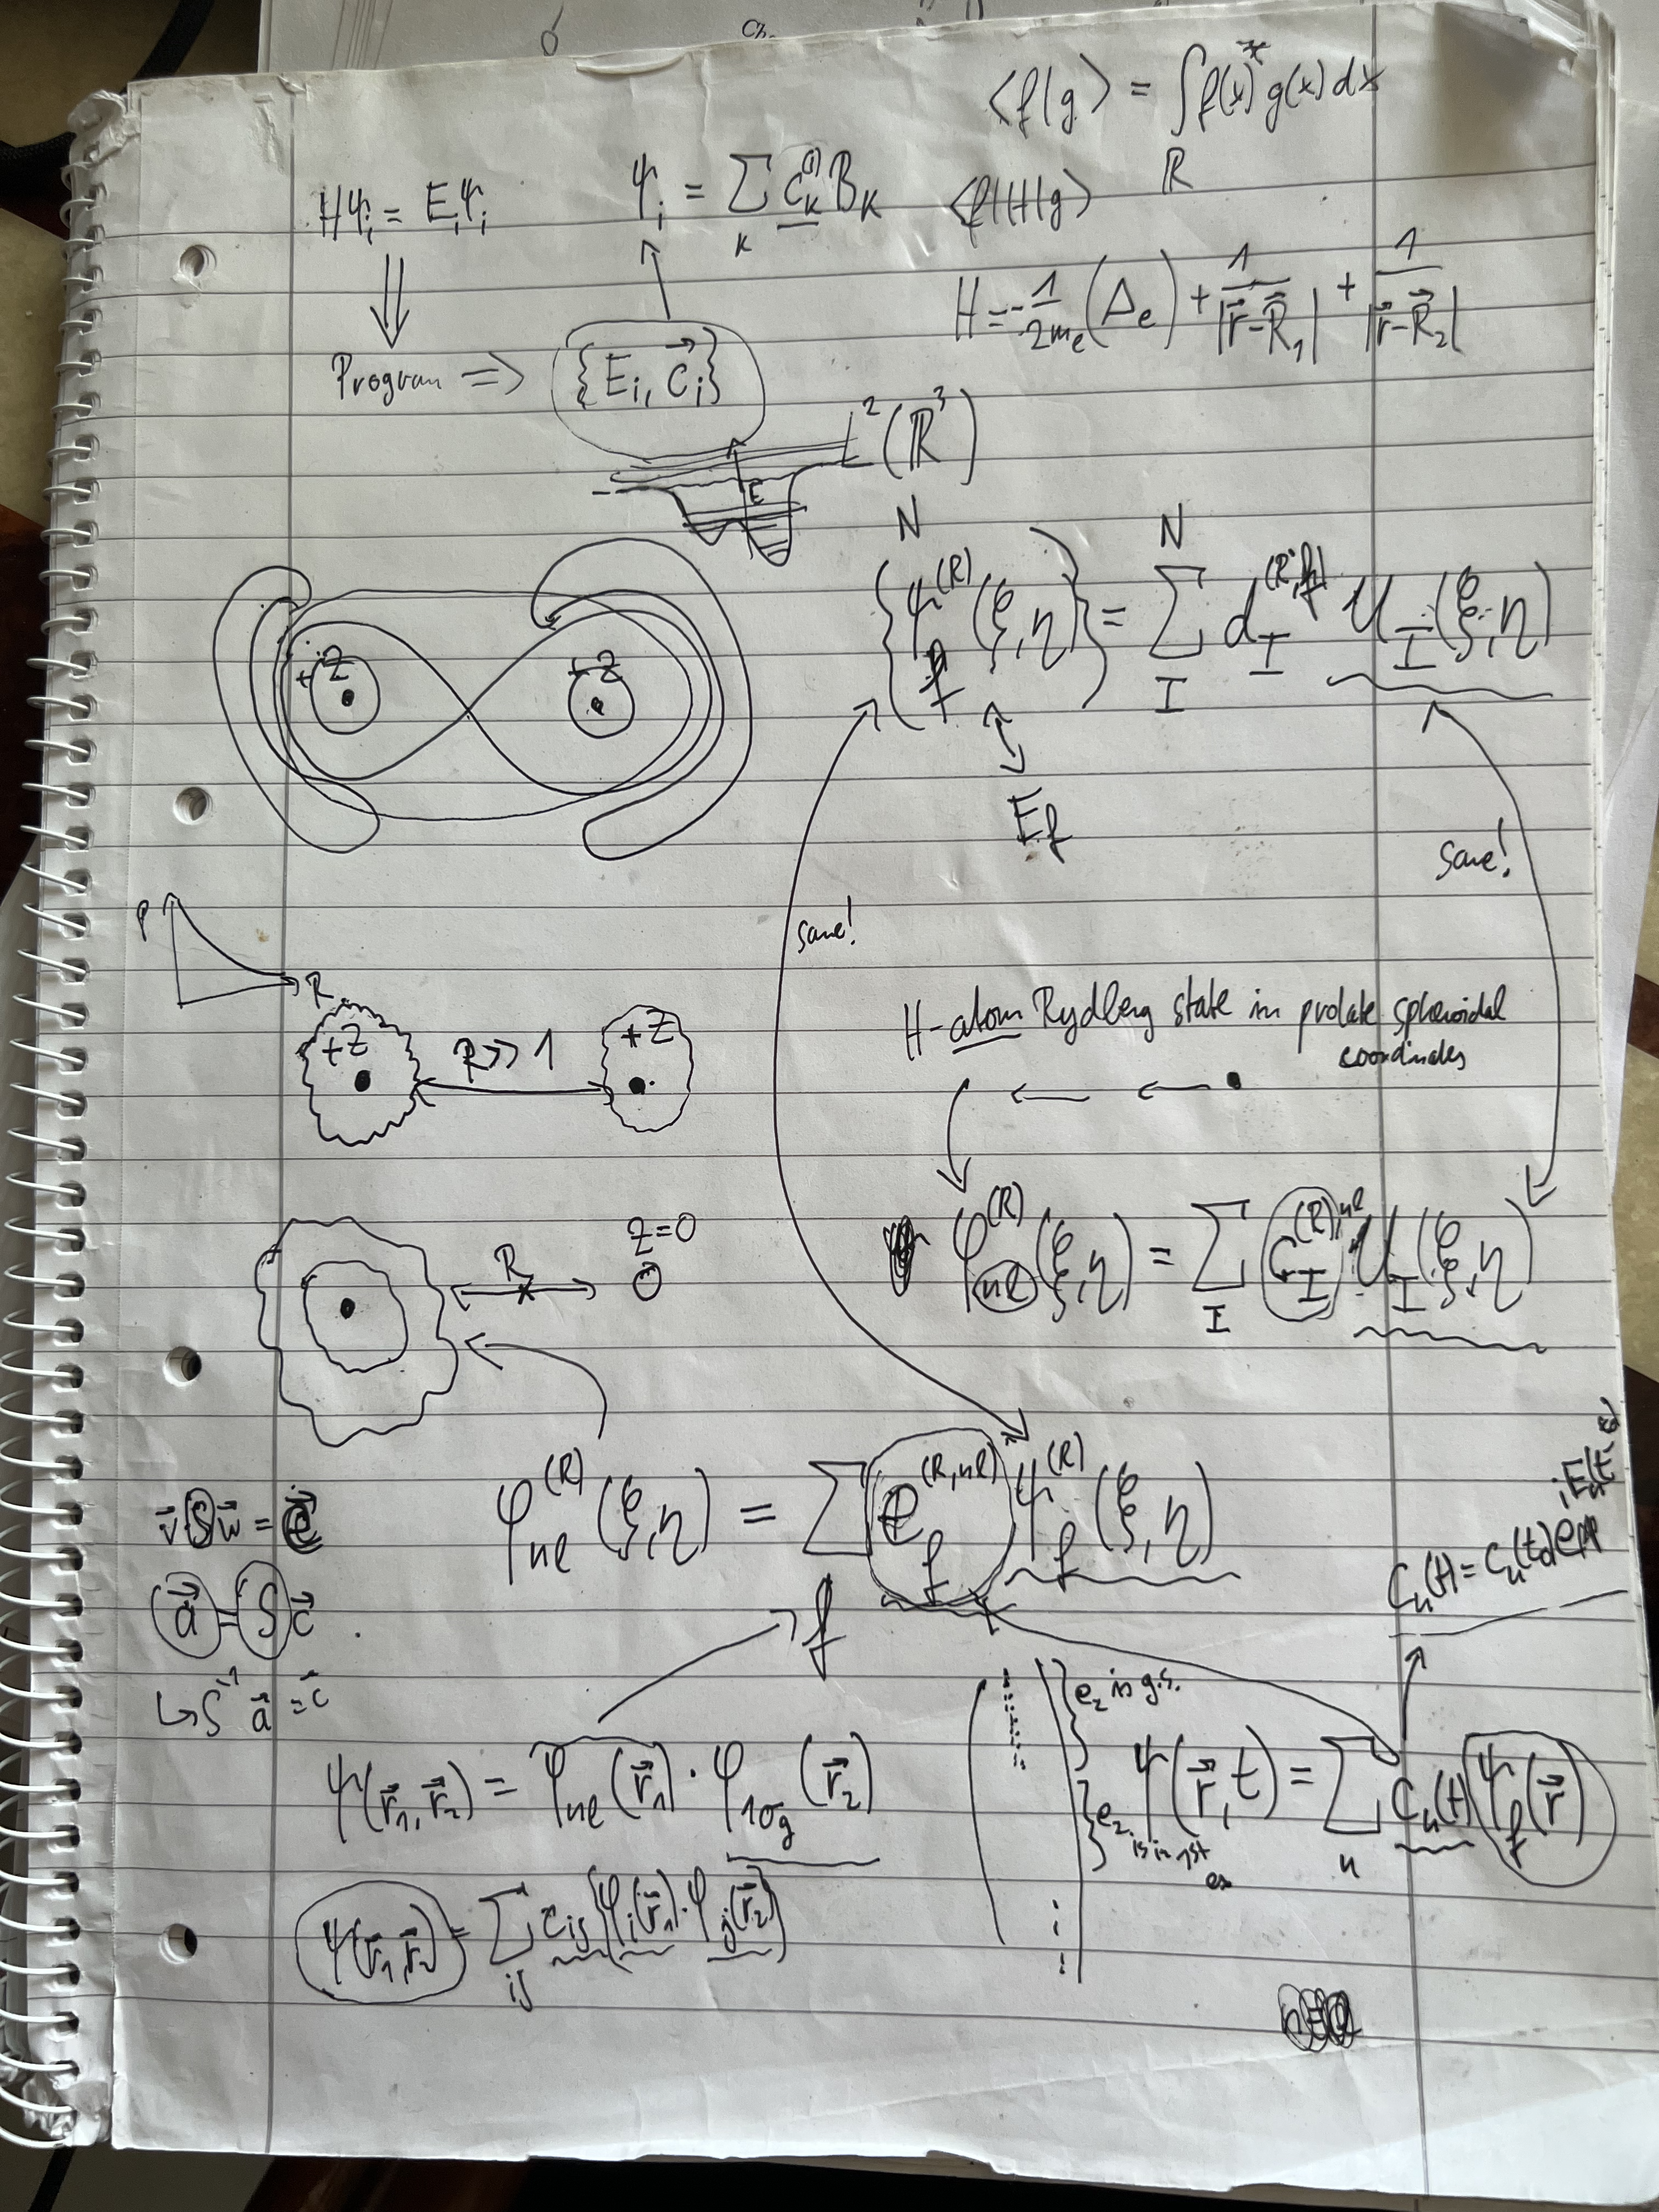
\includegraphics[width=\textwidth]{/Users/JohnnyLin/Desktop/HumboldtProgram/HU_AMO_techincal_report/AMO_report_figures/plan.png}
  \caption{hand written plan}
  \label{fig:plan}
\end{figure}


%
%=====================================================================
%
\printbibliography

%
%=====================================================================
%
\end{document}  % end of the document
%
